\chapter{Konwolucyjne sieci neuronowe}
Konwolucyjne sieci neuronowe (ang. Convolutional Neural Networks)
\section{Zarys historyczny}
\section{Przykłady współczesnych topologii}
\subsection{AlexNet}
Sieć AlexNet, której nazwa pochodzi od imienia głównego twórcy tej architektury Alexa Krizhevsky, zawiera blisko 60 milionów parametrów i 650 tysięcy neuronów. Architekturę zaprezentowano na Rys. \ref{AlexNetTopology}
\begin{figure}[h!]
	\centering
	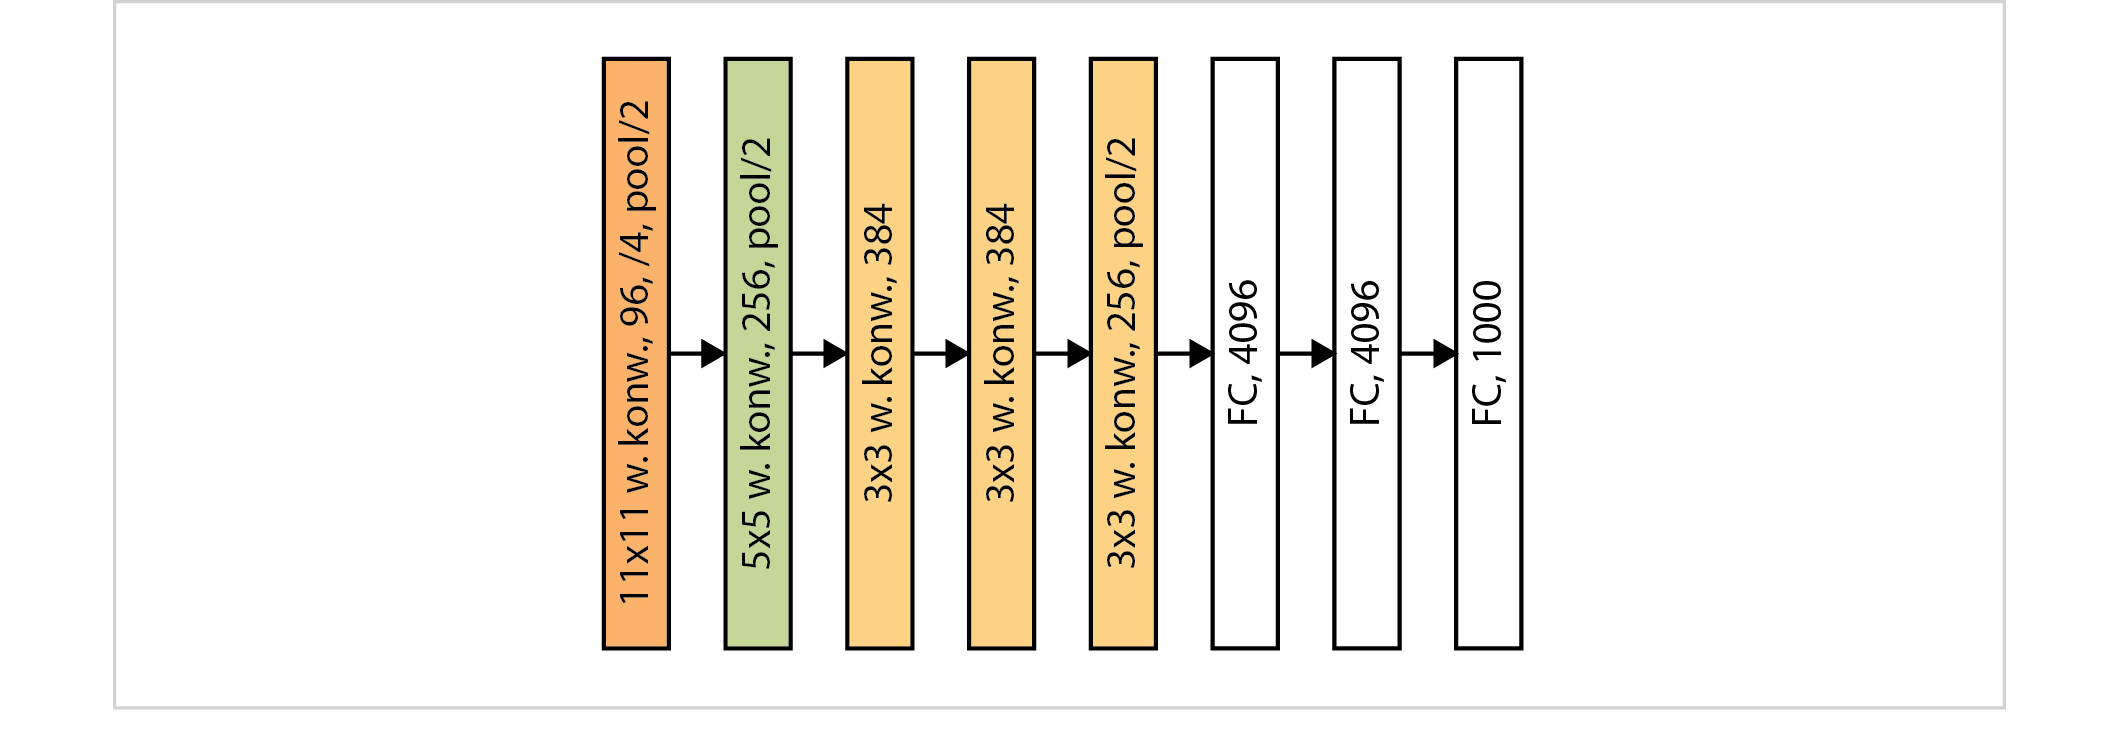
\includegraphics[width=0.55\textwidth]{figures/AlexNet.png}
	\caption{Topologia architektury AlexNet.}
	\label{AlexNetTopology}
\end{figure}

W skład topologii wchodzi pięć warstw konwolucyjnych i trzy typu fully-connected. Po pierwszej, drugiej i piątej warstwie konwolucyjnej występują operacje typu max-pool, stosowane do obszaru 2$\times$2. 

Pierwsza warstwa konwolucyjna przyjmuje na wejściu dane o wymiarze 227$\times$227$\times$3, na których wykonywana jest operacja splotu z 96 filtrami z jądrem splotu o wymiarach 11$\times$11$\times$3 i krokiem 4. W rezultacie (uwzględniając również operacje max-pool) objętość wynikowa przekazywana do kolejnej warstwy ma wymiar 27$\times$27$\times$96. W drugiej warstwie konwolucyjnej wykonywana jest operacja splotu z 256 filtrami z jądrem o wymiarach 5$\times$5$\times$96. Wymiar objętości wynikowej zostaje ponownie zredukowany poprzez operacje max-pool do 13$\times$13$\times$256. Kolejne 3 warstwy konwolucyjne są połączone bezpośrednio ze sobą. Trzecia warstwa zawieraja 384 filtry o wymiarze 3$\times$3$\times$256, w skład czwartej wchodzą 384 filtry o wymiarze 3$\times$3$\times$384, a w piątej znajdują się 256 filtry ponownie o wymiarze 3$\times$3$\times$384. Końcowe dwie warstwy typu FC zawierają po 4096 neuronów, a ostatnia zawiera tyle neuronów ile klas występuje w ostatecznym podziale - w oryginalnej pracy było to 1000 [AlexNet].

Przykładowa implementacja algorytmu przetwarzania sygnału wejściowego przez pierwszą warstwę sieci wygląda następująco: 
\begin{enumerate}
\item Z danych wejściowych o wymiarze [227$\times$227$\times$3] wybierany jest co czwarty blok (zarówno wzdłuż wysokości jak i szerokości) o wymiarach [11$\times$11$\times$3]. Punkty krawędziowe, które stanowią margines potrzebny do wyliczenia splotu są zazwyczaj pomijane. W rezultacie otrzymywanych jest 217 punktów w każdym rzędzie i w kolumnie, w których mieści się [55$\times$55] tj. 3025 bloków.
\item Zarówno 11$\times$11$\times$3 = 363 wagi znajdujące się w 96 filtrach jak i wartości 363 punktów obrazowych znajdujących sie 3025 blokach są przedstawiane w postaci macierzy $A$ o wymiarach [96$\times$363] i $B$ o wymiarach [363$\times$3025].
\item liczony jest iloczyn skalarny w postaci A$^\intercal$B = $C$, gdzie nowa, wyjściowa macierz $C$ ma wymiar [96$\times$3025].
\item Resultat w postaci macierzy $C$ ponownie przewymiarowywany jest na postać [55$\times$55$\times$96].  
\end{enumerate} 

Praca nad architekturą wprowadziła kilka nowości w stosunku do poprzednich architektur takich jak LeNet usprawniając trening sieci.
-ReLU
-MultiGPU
-LRN
-dropout



\subsection{GoogleNet}
\subsection{ResNet}
\subsection{Złożenia}
\section{Zastosowania w medycynie}
\section{Problem nadmiernego dopasowania}
\section{Problem redukcji wymiarowości}